\section{VoLTE传输协议分析}
\label{chap:backinfo:rtp}

%VoLTE实在RTP协议的基础上实现的,RTP自身有一些特征
RTP是VoLTE的应用层协议,通过主动丢包构建时间隐通道,需要结合协议特征进行实现调制与解调。
%在这里进行的分析,如何利用这些特征,构建时间隐通道
RTP协议中,存在具有随机性的字段及结构,利用其随机性能够有效提升时间隐通道的保密性。

\subsection{RTP数据包结构}
\label{chap:backinfo:rtp:struct}

%RTP是怎样的标准,数据包等层次解析
RTP以UDP为传输层协议,避免了类似TCP的握手及挥手过程,也不会受到传输控制的影响。因此,RTP在传输延迟及响应时延方面具有较大优势,在实时音视频通话、互联网实时应用中广泛应用\nupcite{6923336}。根据数据包的层次结构,IP数据包的负载是UDP数据包结构,UDP数据包的负载是RTP数据包结构。由于当前以太网的最大传输单元(MTU)通常设定为{1500\ Bytes},IPv6网络下IP包头长度通常为{40\ Bytes},UDP包头通常为{8\ Bytes},RTP包头通常为{12\ Bytes},所以RTP的数据负载通常不超过{1440\ Bytes}\nupcite{6269462}。因此,视频数据帧必须分包传输,大大增加了视频数据包的数量。

\insertFigure{
	\begin{figure}[htbp]
		\centering
        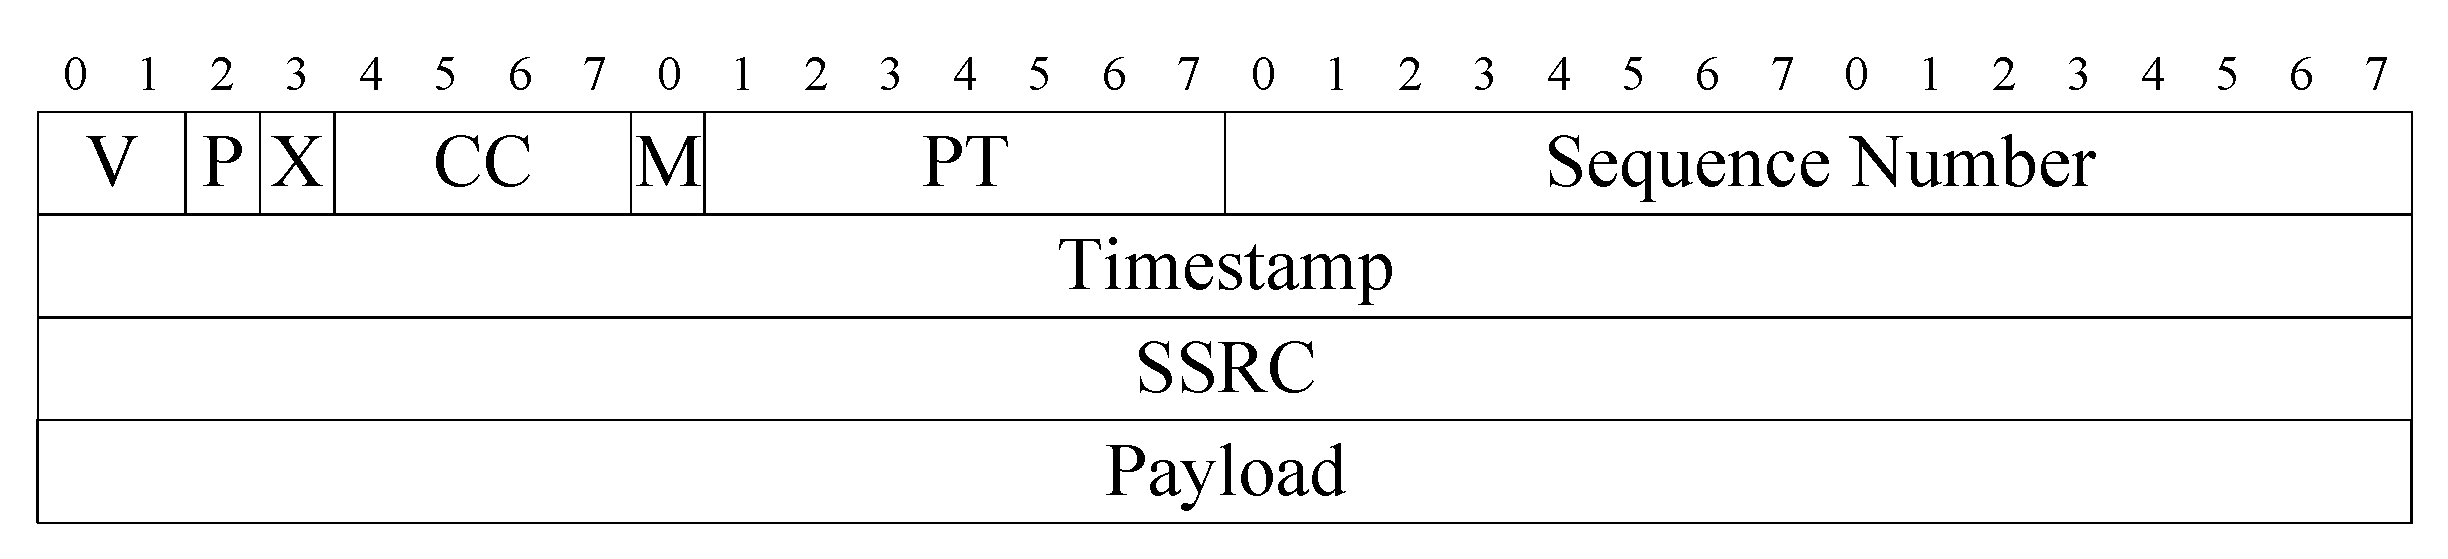
\includegraphics[width=0.9\textwidth]{chapters/chapter2/figures/rtp-header.pdf}
        \caption{RTP包头结构示意图}\label{fig:2:rtp-header}
	\end{figure}
}

%RTP头的组成
VoLTE中常见的RTP包头结构如图\ \nref{fig:2:rtp-header},在包头中存在固定的字段,如V({Version})表明RTP协议版本,M({Marker})标识视频帧分包的终止位置,PT({Payload Type})指明数据负载类型\nupcite{6923336}。

\subsection{随机字段}
\label{chap:backinfo:rtp:random}

%RTP参数中,包含哪些随机生成的字段
RTP数据包头中,存在一些特殊的字段,其取值在标准中有特殊要求。

%SSRC、TimeStamp,生成的效果
图\ \nref{fig:2:rtp-header}中的{Sequence Number}字段,用于标识一次通话中的数据包顺序,按照步长为1的规律递增。数据包序号的初始值要求随机生成,从而抵御已知明文攻击。

图\ \nref{fig:2:rtp-header}中的{Timestamp}字段,反映了采样时间的间隔,便于接收方在网络抖动时,按照正确的时序还原数据。该字段的初始值也应该为随机值,并且在不同的传输流中,通过步长体现采样时间的差异\nupcite{6156339}。

图\ \nref{fig:2:rtp-header}中的{SSRC}({Synchronization Source identifier})字段,用于标记数据源。该字段取值必须随机生成,从而避免在一次RTP会话中出现相同的{SSRC},并且在数据源改变后重新生成。{SSRC}字段的设计,实现了字段值与数据流的对应,具有流量标识的功能\nupcite{6222709}。

%用于时间隐通道的秘钥及随机特征生成,保证保密性
时间隐通道作为隐蔽传输方法,其传输的隐蔽消息不应被破解或截获。借助RTP中的随机字段,迭代伪随机数生成算法,为每次传输生成随机扰动,从而有效防范监听者对隐蔽消息的破解。

\subsection{RTP丢包处理}
\label{chap:backinfo:rtp:dropout}

%RTP及应用中,对于丢包事件的处理
根据RTP数据包的层次结构,丢包影响需要综合各层次进行分析。对于IP层,由于无法感知丢包事件,因此不会进行丢包处理;由于UDP本身不具备重传及确认机制,无法保证数据包送达,也不存在重传行为;RTP重点在于实时性,而重传会导致传输阻塞,从而破坏实时性效果,因此只在RTCP数据包中反馈网络质量\nupcite{6423613,5478577,6894614}。

%丢包不重传,序号保证自增,是主动丢包方法的基础
RTP中数据包序号不重复、丢包后不重传,是基于主动丢包时间隐通道的构建基础。对于时间隐通道,在发送方丢弃的数据包,接收方一定可以感知到丢包事件,因此具备消息传输基础。同时数据包序号具有同步时钟的效果,时间隐通道根据序号范围划分丢包区间,即可确保解调过程与调制过程的一致性。